\chapter{Discussion}\label{chapter:discussion}

One aim of the master thesis was to investigate whether GraphQL with a shared caching layer and query reduction can improve performance in micro-frontend architectures. The improvement should be accomplished using a single caching layer for all micro-frontends and a mechanism to reduce queries by utilizing the in-memory cache structure. The technology-agnostic and prototypical implementation of the micro-frontends is further discussed in this chapter. The results of evaluating the caching improvements of the prototypical micro-frontend implementation architecture are also discussed in this chapter. The findings of Chapter \ref{chapter:results} are used to make a statement about the hypothesis from Chapter \ref{chapter:introduction}. The following sections focus on discussing the results regarding request size and response size. The chapter closes by comparing the total time to fetch all responses from the \ac{BFF}.

\section{Request Size}\label{section:discussion:request-size}

This section compares the different measurements of the request sizes from Chapter \ref{chapter:results}. Figure \ref{fig:discussion:request-size} displays the results from the previous sections \ref{section:results:comparison-first-journey} and \ref{section:results:comparison-second-journey} as a bar chart for better comparison. As shown in the figure for the first user journey, the differences in request sizes are not very significant. The first approach, with no query reduction and no shared cache, is the largest and executes 11 more requests than the other two. These 11 extra GraphQL queries make up the total difference from the second approach with just the shared caching layer because the queries are not reduced using the cache. The difference between the second and the third approach is only 1.65 KB. 

\bigskip

\noindent The second user journey shows a similar result. Compared to the first, 25 requests are omitted in the second approach by just using a shared caching layer. These differences in network requests result in a more significant difference in request sizes, about 6.07 KB. However, the difference from the second approach to the third approach is slight, as it is again about 2.17 KB. The difference between the second and third approaches comes only from the omitted fields in the query. The difference of 2.17 KB is relatively tiny compared to the 37 GraphQL queries that were executed against the \ac{BFF}.

\bigskip

\noindent Therefore, the query reduction does not significantly improve performance by reducing the size of the requests compared to just using the shared caching layer.

\begin{figure}[H]
  \centering
  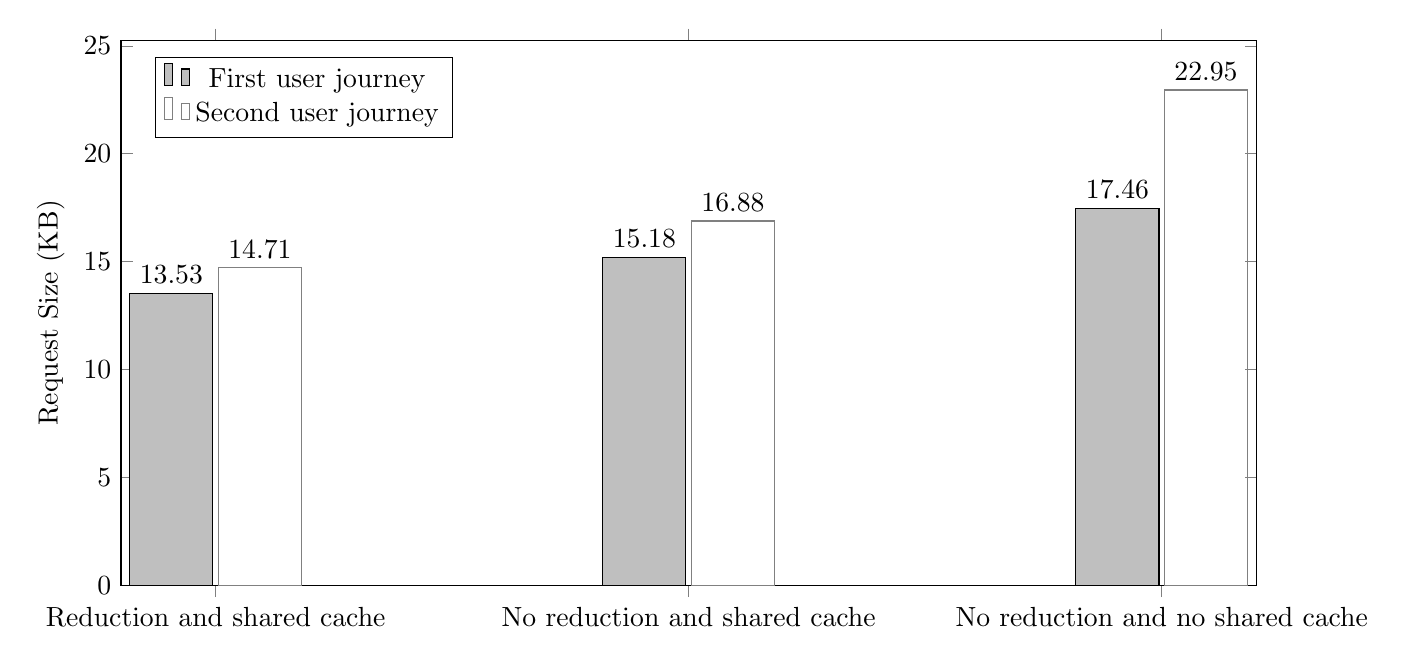
\begin{tikzpicture}
    \begin{axis}[
      ymin=0,
      ybar,
      legend pos=north west,
      ylabel={Request Size (KB)},
      xtick=data, 
      symbolic x coords={Reduction and shared cache, No reduction and shared cache, No reduction and no shared cache}, 
      nodes near coords align={vertical},
      nodes near coords,
      height=8.5cm,
      width=16cm,
      bar width=30pt,
      cycle list={
        {fill=lightgray, draw=gray}
      },
    ]
    \addplot coordinates {(Reduction and shared cache, 13.53) (No reduction and shared cache, 15.18) (No reduction and no shared cache, 17.46)};
    \addplot coordinates {(Reduction and shared cache, 14.71) (No reduction and shared cache, 16.88) (No reduction and no shared cache, 22.95)};
    \legend{First user journey, Second user journey}
    \end{axis}
  \end{tikzpicture}
  \caption{Request size comparison between the three approaches.}\label{fig:discussion:request-size}
\end{figure}

\noindent The following section compares the response sizes of the GraphQL \ac{API} for the three approaches.

\section{Response Size}\label{section:discussion:response-size}

This section compares the three approaches' response sizes from the GraphQL API. Figure \ref{fig:discussion:response-size} displays the results already shown in the previous sections \ref{section:results:comparison-first-journey} and \ref{section:results:comparison-second-journey} as a bar chart for better comparability. Clearly, visible is that the differences in response size are more significant than the difference in request size. As displayed in the figure, the difference between the approach with no query reduction and no shared cache is about 2.35 MB. Therefore, the 11 requests that are omitted by using the shared caching are responsible for more than 2 MB of data that needs to be downloaded unnecessarily. This difference could significantly affect page performance when using a mobile device. The difference between the second and third approaches is only about 62 KB, which is insignificant and does not make a real difference. Saving 62 KB of data in 37 GraphQL queries is not worth the effort of implementing and using the query reduction. 

\bigskip

\noindent The second user journey shows a similar outcome, as the size differences are similar. The second approach in the user journey omits 25 requests compared to the naive first approach. These fewer requests results again in a difference of about 2.35 MB. The second and third approaches have just a 3 KB difference in response sizes. These differences are coming from the omitted fields from queries, which are pretty small compared to the 37 GraphQL queries that are executed against the \ac{BFF}.

\bigskip

\noindent Just like with the request sizes, the query reduction does not significantly improve performance by reducing the size of the responses compared to just using the shared caching layer.

\begin{figure}[H]
  \centering
  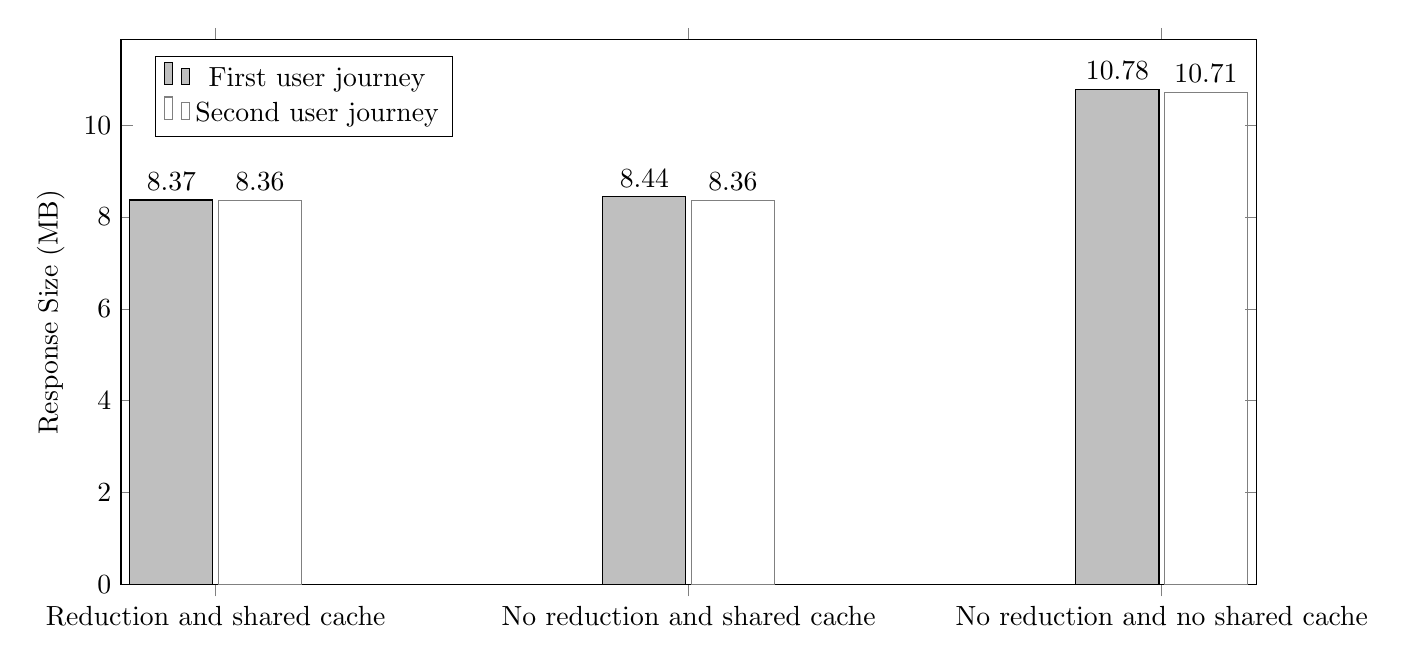
\begin{tikzpicture}
    \begin{axis}[
      ymin=0,
      ybar,
      legend pos=north west,
      ylabel={Response Size (MB)},
      xtick=data, 
      symbolic x coords={Reduction and shared cache, No reduction and shared cache, No reduction and no shared cache}, 
      nodes near coords align={vertical},
      nodes near coords,
      height=8.5cm,
      width=16cm,
      bar width=30pt,
      cycle list={
        {fill=lightgray, draw=gray}
      },
    ]
    \addplot coordinates {(Reduction and shared cache, 8.37) (No reduction and shared cache, 8.44) (No reduction and no shared cache, 10.78)};
    \addplot coordinates {(Reduction and shared cache, 8.361) (No reduction and shared cache, 8.364) (No reduction and no shared cache, 10.71)};
    \legend{First user journey, Second user journey}
    \end{axis}
  \end{tikzpicture}
  \caption{Response size comparison between the three approaches.}\label{fig:discussion:response-size}
\end{figure}

\noindent The following section takes the response into perspectives and compares the response times of the three approaches. This factor is vital because smaller responses lead to faster responses, which is crucial for the user experience.

\section{Response Times}\label{section:discussion:response-times}

It is hard to make accurate comparisons when it comes to measuring the time it takes to fetch the responses from the GraphQL \ac{API}. The network speed can vary significantly over time; therefore, it takes work to make a reproducible comparison. Therefore, the measurement was done using the throttle mode inside the Google DevTools\footnote{\url{https://developer.chrome.com/docs/devtools/}}. The network speed was set to 1.5 Mbps, also named \enquote{fast 3G} preset inside the developer tools. This setting ensures the network speed stays the same for testing all three approaches. The response times were measured three times for every approach, and the mean value was taken to get a neutral value. The preset \enquote{fast 3G} was chosen because it is pretty slow and makes it possible for times to differ more significantly. With faster network speeds, the differences would be more minor and harder to compare. Moreover, 3G is still a typical network speed for mobile connections in many countries.

\bigskip

\noindent This section measures the total time to download every query response from the GraphQL \ac{API} for the three approaches from Section \ref{section:results:performance-measurement}. The measurement should not be misunderstood, because the browser partially loads the resources in parallel. Here only total download time is measured to see how much time is needed to download all the resources in one of the approaches. The measurements were recorded during the user journeys from sections \ref{section:results:comparison-first-journey} and \ref{section:results:comparison-second-journey} alongside the request sizes and response sizes. Therefore the total response times correspond to the measured network sizes from the previous two chapters. The results are measured in seconds and are shown in figure \ref{fig:discussion:response-times}. 

\begin{figure}[H]
  \centering
  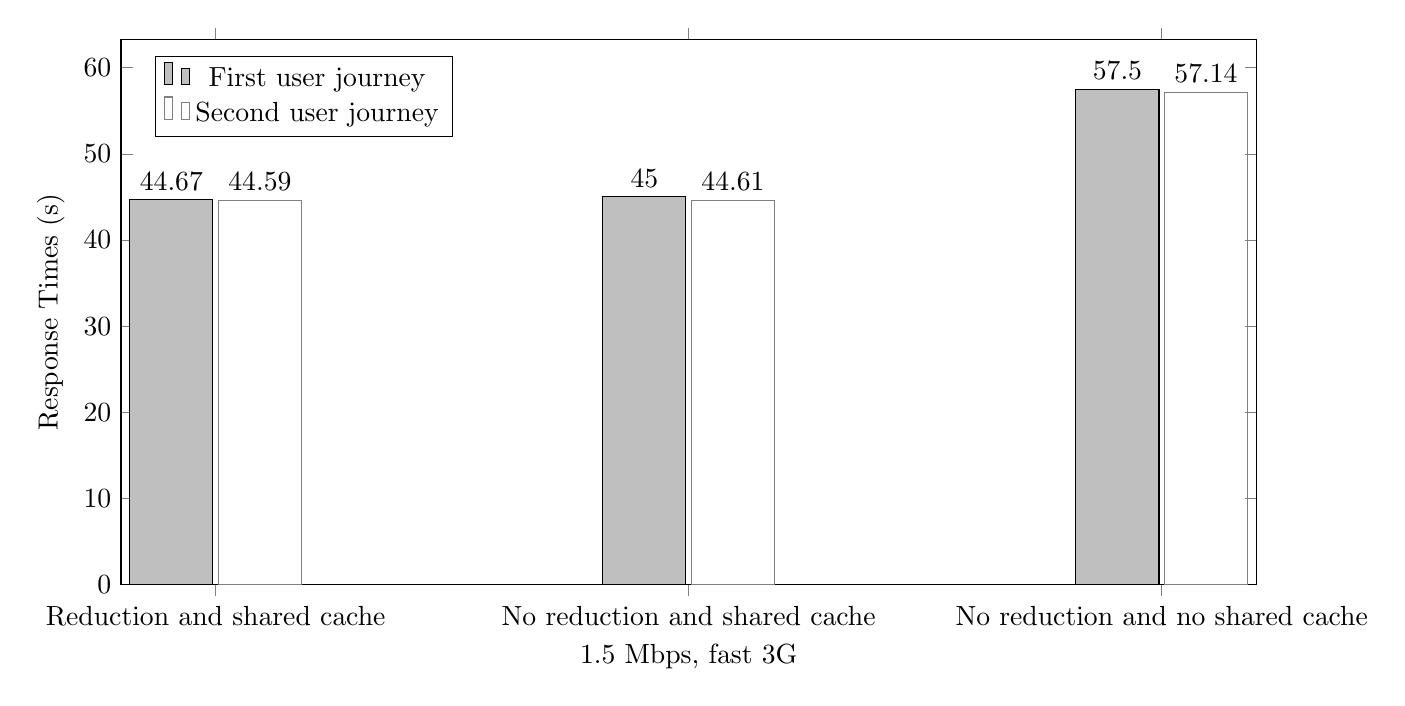
\begin{tikzpicture}
    \begin{axis}[
      ymin=0,
      ybar,
      legend pos=north west,
      ylabel={Response Times (s)},
      xlabel={1.5 Mbps, fast 3G},
      xtick=data, 
      symbolic x coords={Reduction and shared cache, No reduction and shared cache, No reduction and no shared cache}, 
      nodes near coords align={vertical},
      nodes near coords,
      height=8.5cm,
      width=16cm,
      bar width=30pt,
      cycle list={
        {fill=lightgray, draw=gray}
      },
    ]
    \addplot coordinates {(Reduction and shared cache, 44.67) (No reduction and shared cache, 45.00) (No reduction and no shared cache, 57.50)};
    \addplot coordinates {(Reduction and shared cache, 44.59) (No reduction and shared cache, 44.61) (No reduction and no shared cache, 57.14)};
    \legend{First user journey, Second user journey}
  \end{axis}
  \end{tikzpicture}
  \caption{Response time comparison between the three approaches.}\label{fig:discussion:response-times}
\end{figure}

\noindent Like before, the difference between the first and second approaches is quite significant. The second approach for both journeys is about 12 seconds faster than the first approach. The 11, respectively, 25 requests omitted using the shared caching layer are responsible for about 12 seconds of extra download time in the first approach. The results from this measurement correspond to the response size measurements from the previous Section \ref{section:discussion:response-size}. The results for the second and third approaches are practically the same. Reducing 37 queries does not yield the expected results and does not speak in favor of using query reduction.